\subsubsubsection{Bootstrap}
In order to start the application-layer neatly we have to consider the 
dependencies between the entity types exposed in \ref{fig:sd-entity-types-deps}. 
We have also to consider that the application-layer can not decide by itself 
when is time to boot, indeed the application-layer is instructed by the 
middleware-layer. The bootstrap of the application-layer needs a \textit{master} 
process which will create the entities based on the configuration provided by 
the middleware-layer. Considering the dependencies:
\begin{itemize}
  \item The \textit{reactive} entities have to start before the \textit{active} 
ones, because the latter use the former; 
  \item The \textit{passive} entities have no particular dependency. Since 
they are stateless and belong to \textit{reactive} entities (the road signs 
belong to roads) they will be instantiated along with them.
\end{itemize}

\begin{figure}[H]
  \centering
  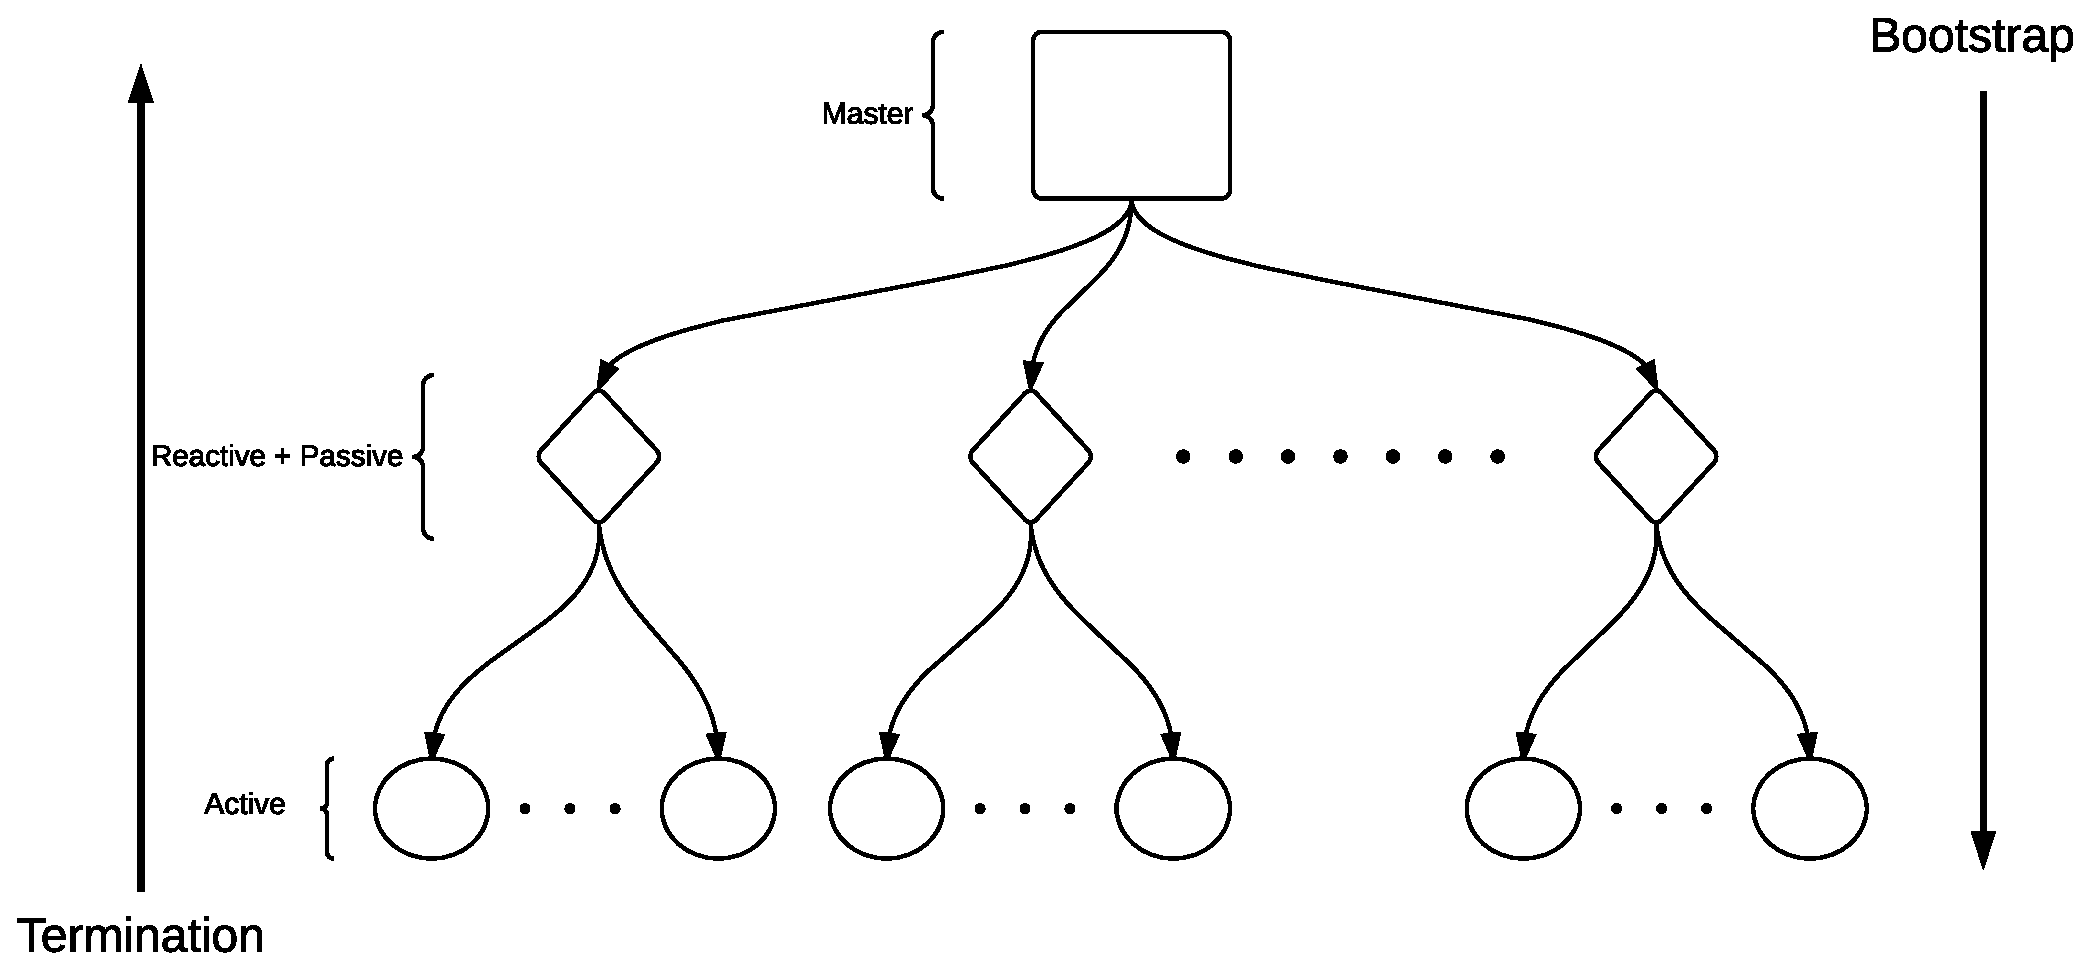
\includegraphics[width=\columnwidth]{sections/images/solution/app_proc_tree.eps}
  \caption{Application process tree}
  \label{fig:app-proc-tree}
\end{figure}

At the end of the bootstrap process the \textit{master} will notify the 
middleware-layer that the bootstrap has completed successfully. If the 
\textit{master} crashes before the bootstrap has completed then 
the middleware-layer will notice that because the timeout 
attached to the \texttt{app.boot} call expires. 


